\chapter{Results}\label{sec:results}

\section{Filtering out noise}\label{sec:noise}
After the tracking and stitching steps are completed, the algorithm results can
still be improved by filtering the results. A large improvement was
achieved by requiring a certain sea surface temperature at TC genesis.
\subsection*{Sea Surface Temperature Criterion}
As outlined in Sec.~\ref{sec:physics} the TCs need warm ocean water as an
energy source, especially when they form. It has been shown that the large
majority has a SST over 25.5\degree C \cite{sst-paper}. Therefore it is
expected that no reasonable TCs are filtered out when requiring a genesis SST
of at least 24\degree C. However as can be seen in Fig.~\ref{fig:sst-effect}
a large part of the unwanted tracks in the North of the domain are removed.
% TODO use figures here and in general with reasonable and elaborated parameters only
\begin{figure}[ht]
	\begin{minipage}[t]{0.48\textwidth}
		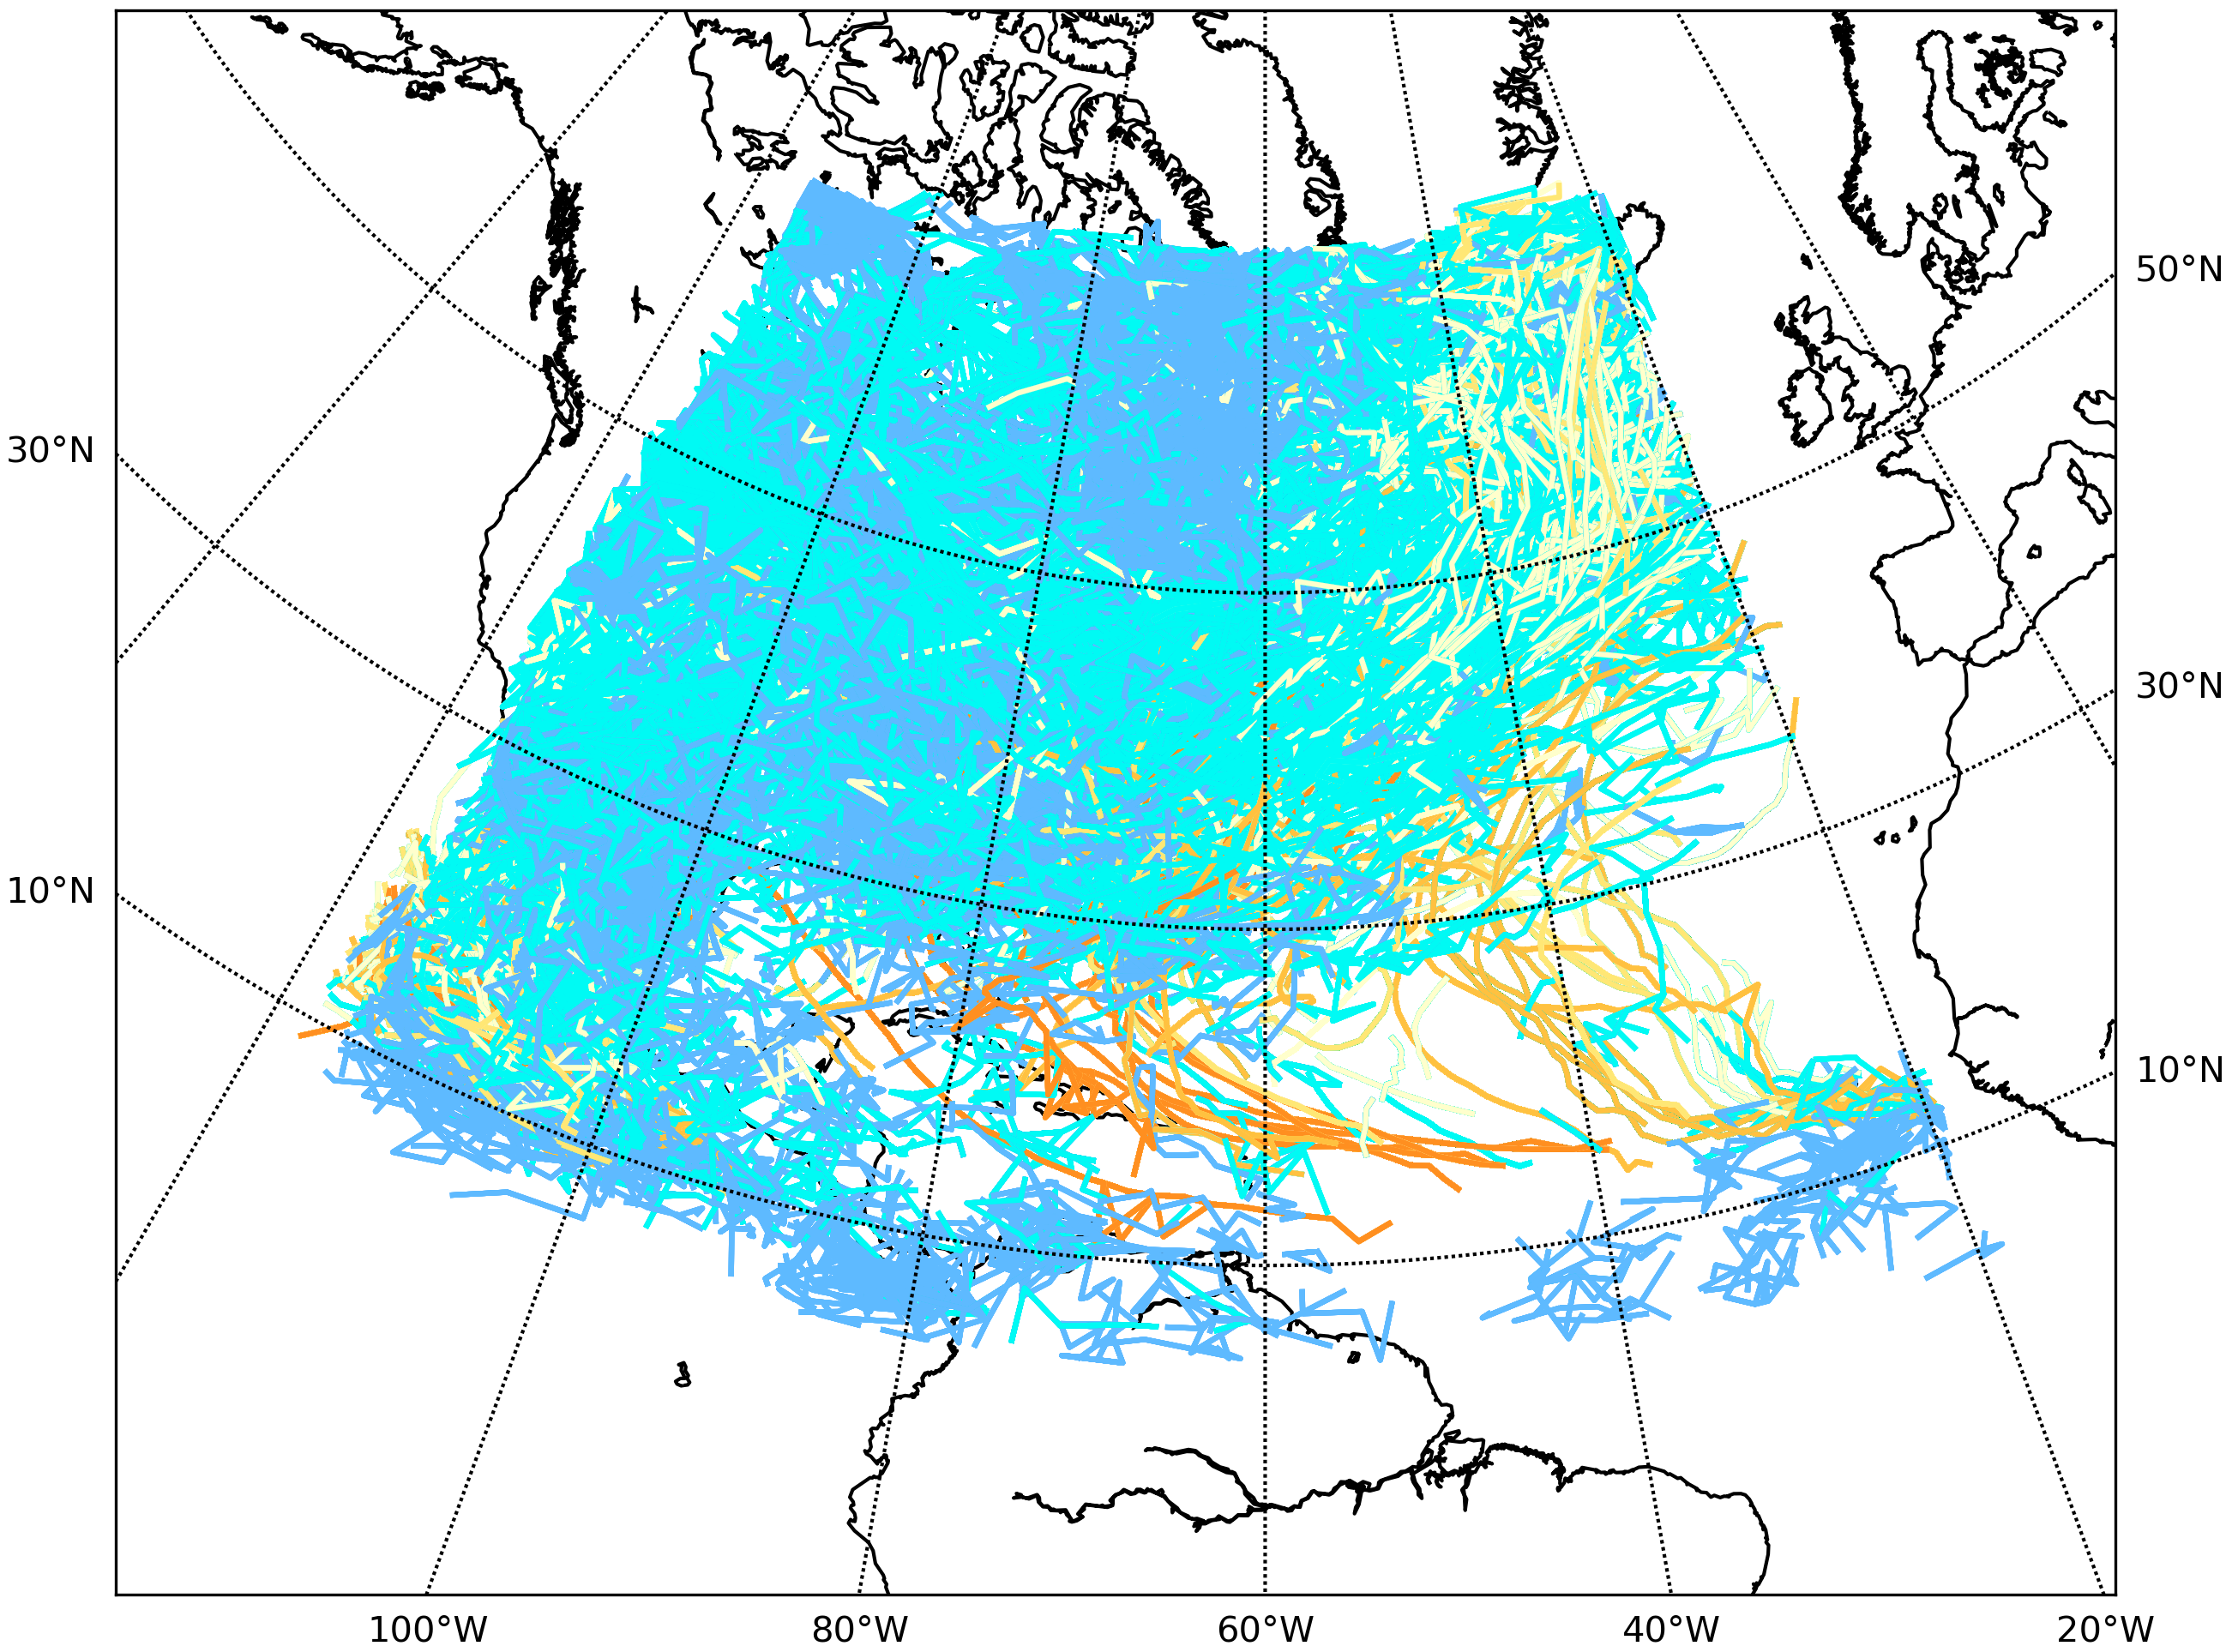
\includegraphics[width = \textwidth]{img/all_tracks.png}
	\end{minipage}
	\hfill
	\begin{minipage}[t]{0.48\textwidth}
		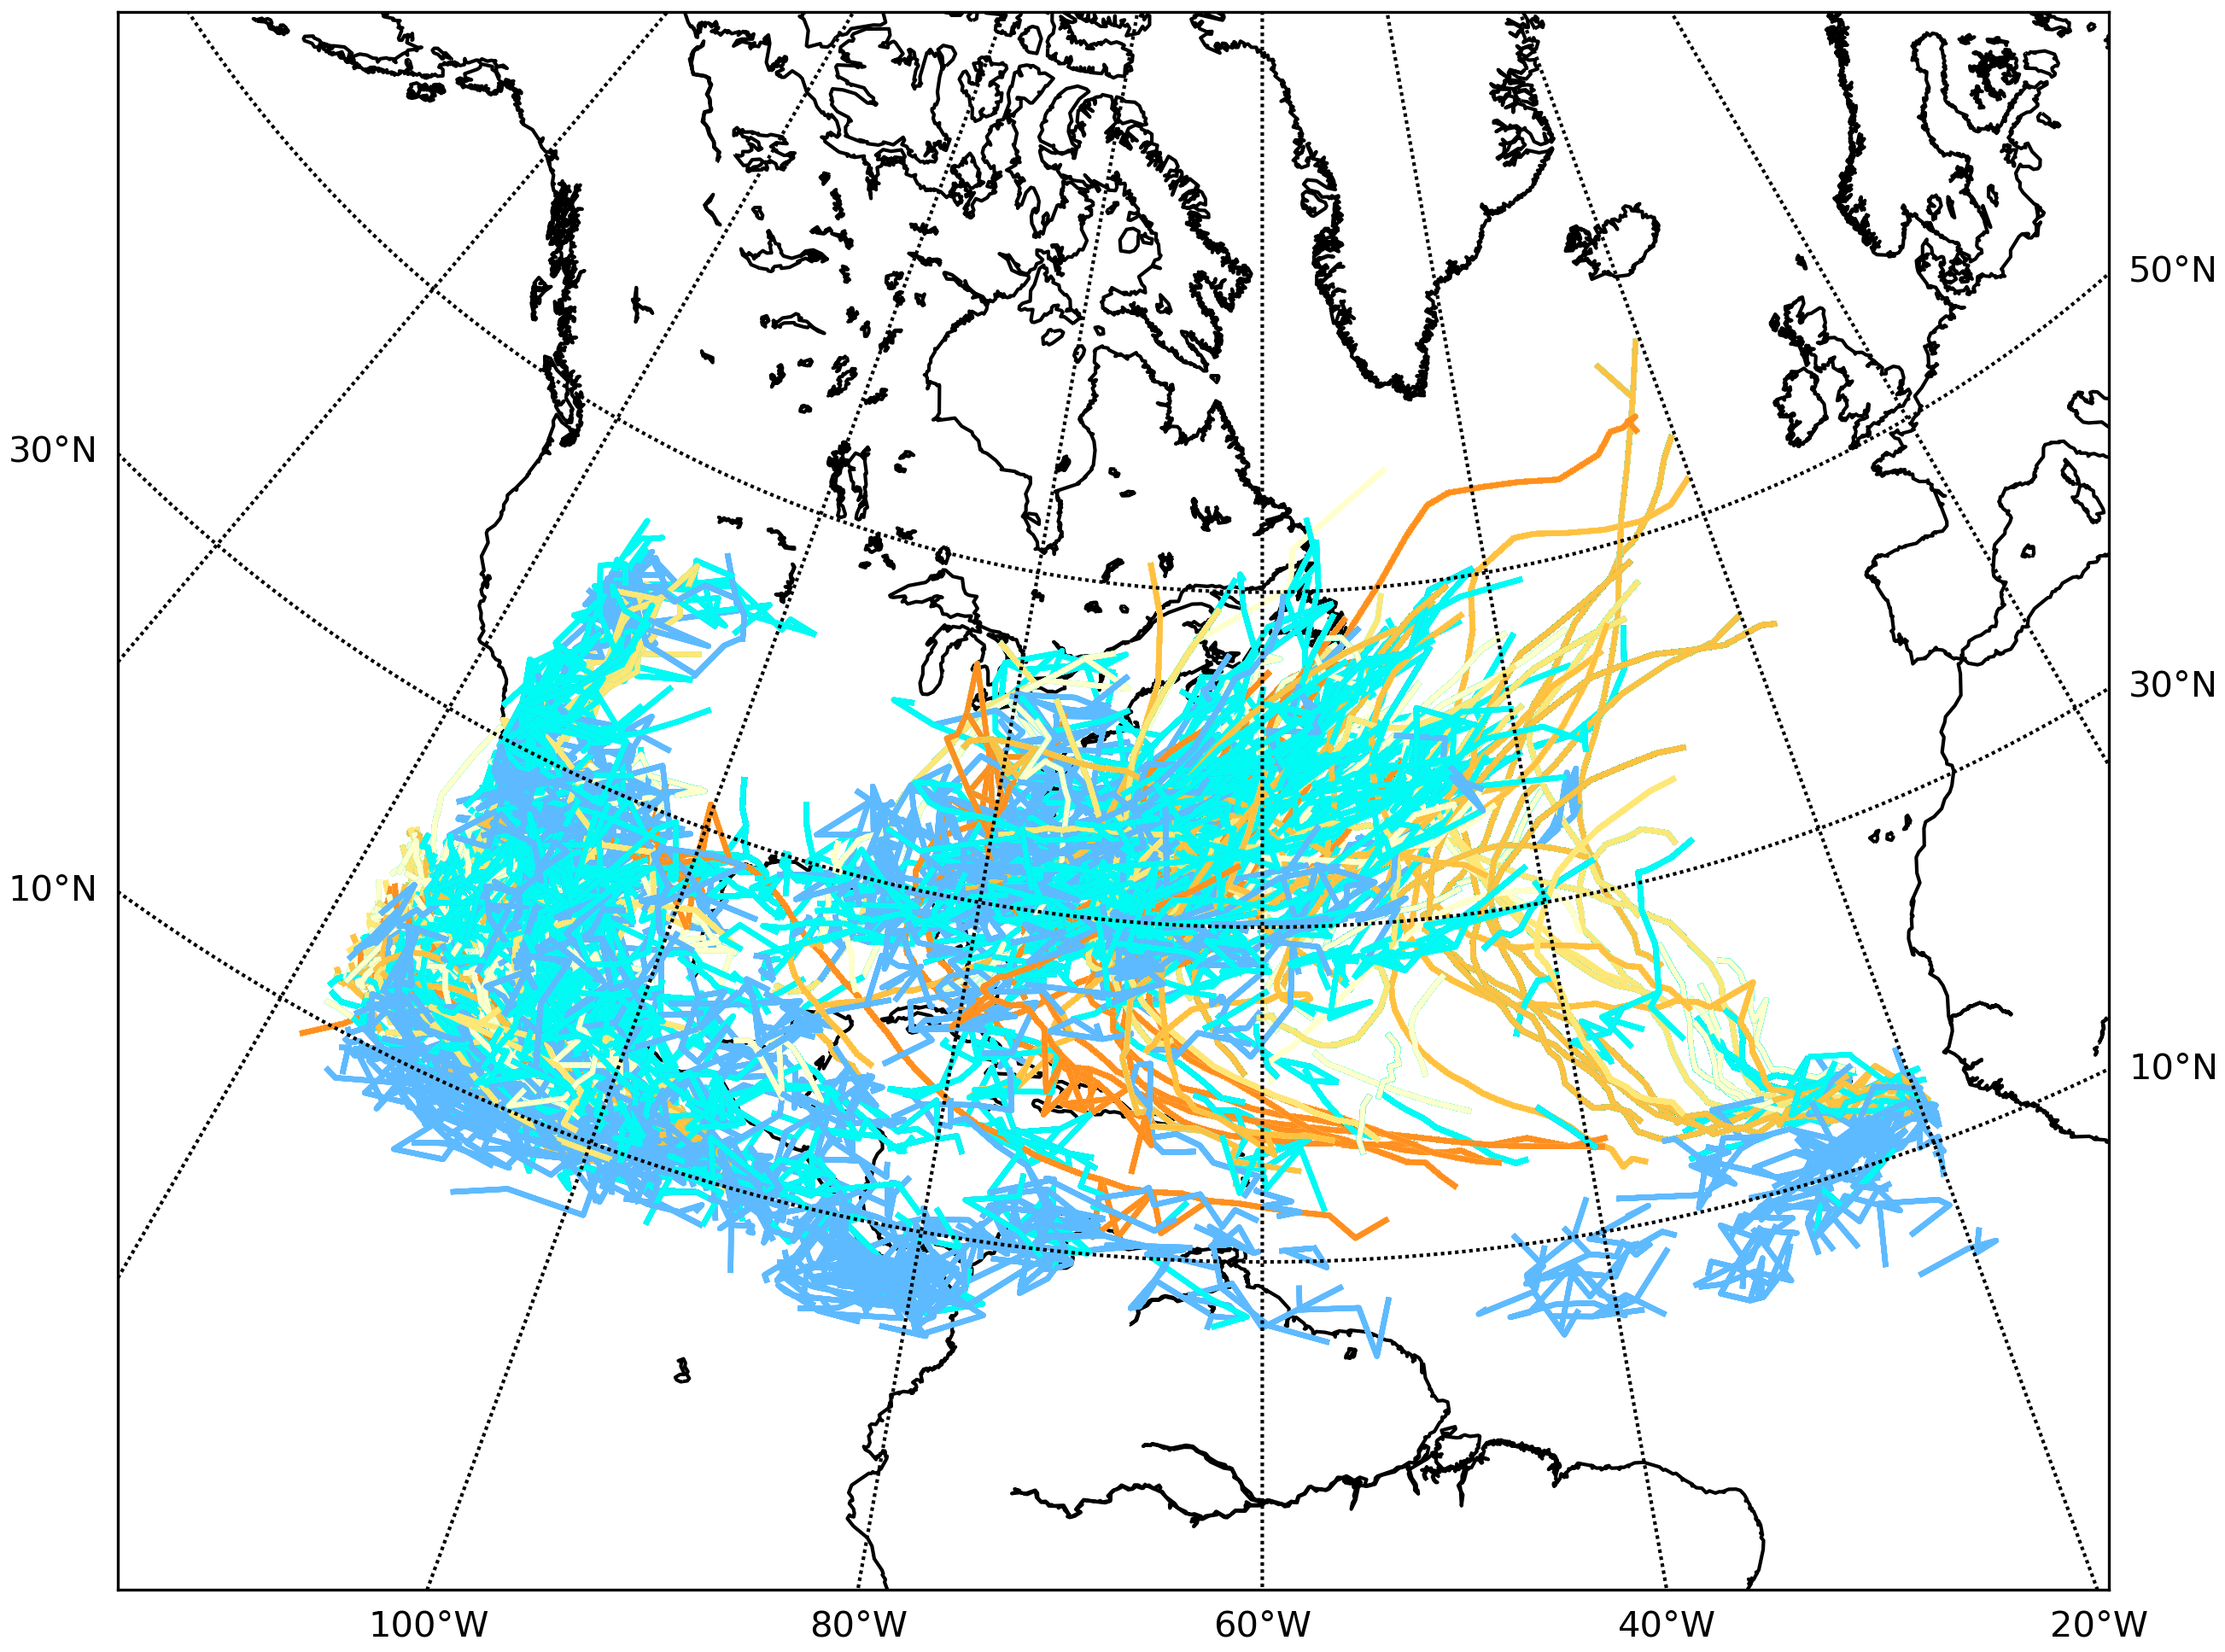
\includegraphics[width = \textwidth]{img/all_tracks_sst.png}
	\end{minipage}
	\caption{Comparison of all tracks without and with the SST criterion on the left and right}
	\label{fig:sst-effect}
\end{figure}

\subsection*{Analysing geographically unreasonable tracks}
Even with the application of the SST-criterion, unreasonable TC tracks remain. For instance the tracks over Wyoming shown in Fig.~\ref{fig:rogue-tracks} should not be so frequent. To determine the parameters responsible for this, the 20 parameter combinations that account for the large majority of these, share the common feature that they all corresponded to the same weak warm core criterion. They had a \textbf{temdif} of \unit[0.5]{\degree C} and a \textbf{temdis} of \unit[400]{km}. Therefore if only a very low temperature difference is required for an area that can be larger than smaller sized TCs, low pressure systems that do not correspond to tropical cyclones are tracked. While this may not be surprising, it does emphasise the importance of a well trimmed warm core criterion.
\begin{figure}[ht]
	\centering
	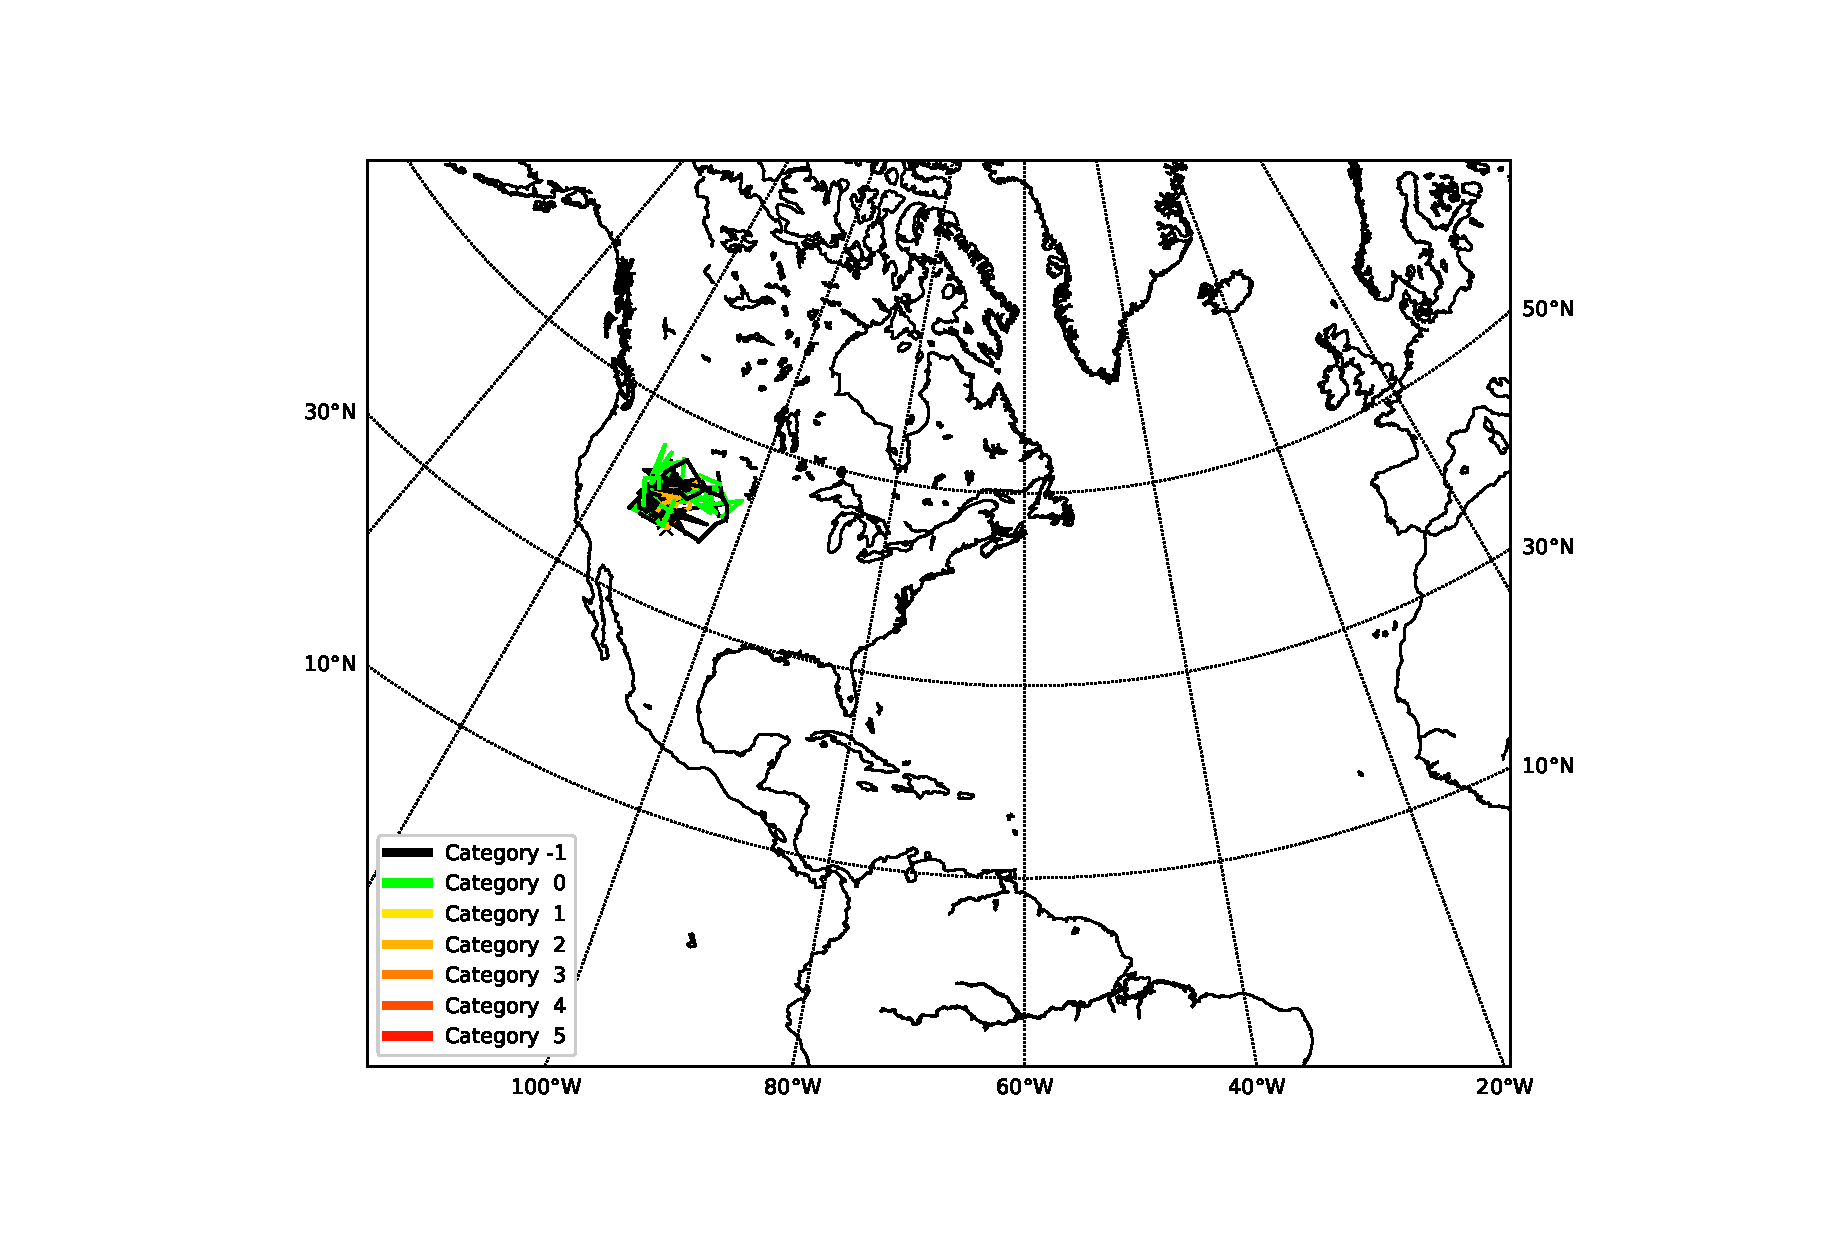
\includegraphics[width=0.7\textwidth]{img/rogue_tracks.eps}
	\caption{Set of unreasonable tracks over Wyoming and the surrounding states}
	\label{fig:rogue-tracks}
\end{figure}
\section{Validating Results}
In Sec.~\ref{sec:noise} it was found that with a sufficiently strong warm core condition the tracks appear in reasonable areas. Before comparing the algorithm output for different parameter combinations, it still remains to be shown that the produced tracks actually follow TCs and not other low pressure systems. For that purpose ten different storms were randomly chosen. For these storms the radial, tangential and vertical wind and the sea level pressure were visualised in the azimuthal mean. It was found that all storms qualitatively exhibit the physically expected structure that was described in Sec.~\ref{sec:physics}. The resulting plots for a representative storm can be seen in Fig.~\ref{fig:azimean}.

\begin{figure}[b]
\centering
\begin{subfigure}{.5\linewidth}
    \centering
    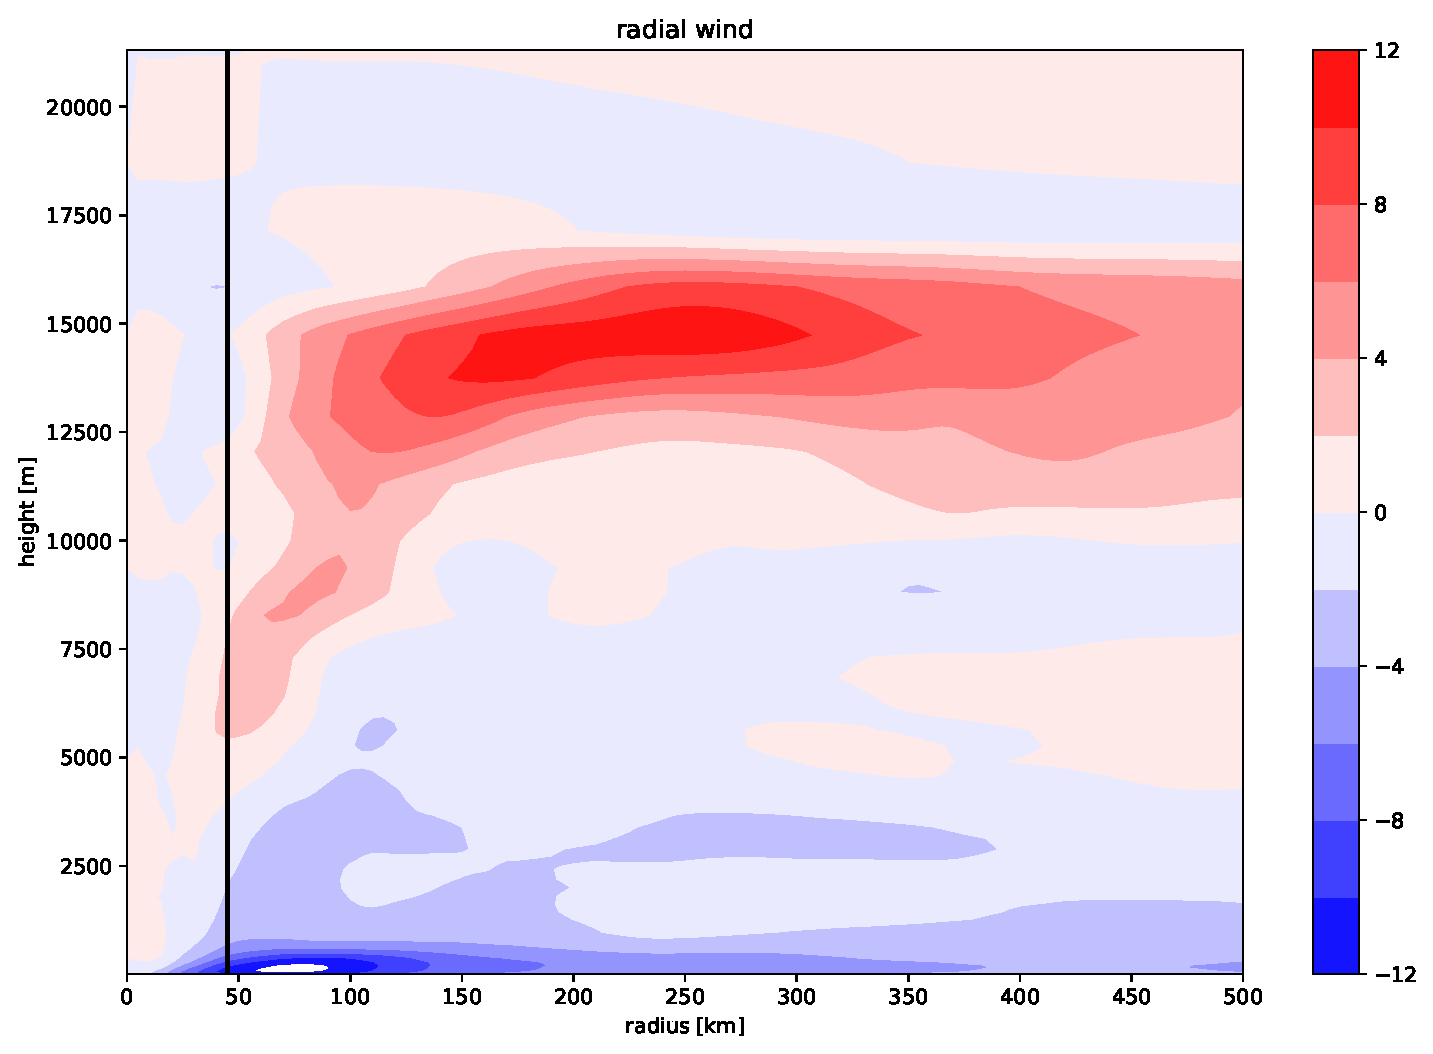
\includegraphics[width=0.75\linewidth]{img/tight09279566radwind20130706T120000Z.eps}
\end{subfigure}%
\begin{subfigure}{.5\linewidth}
    \centering
    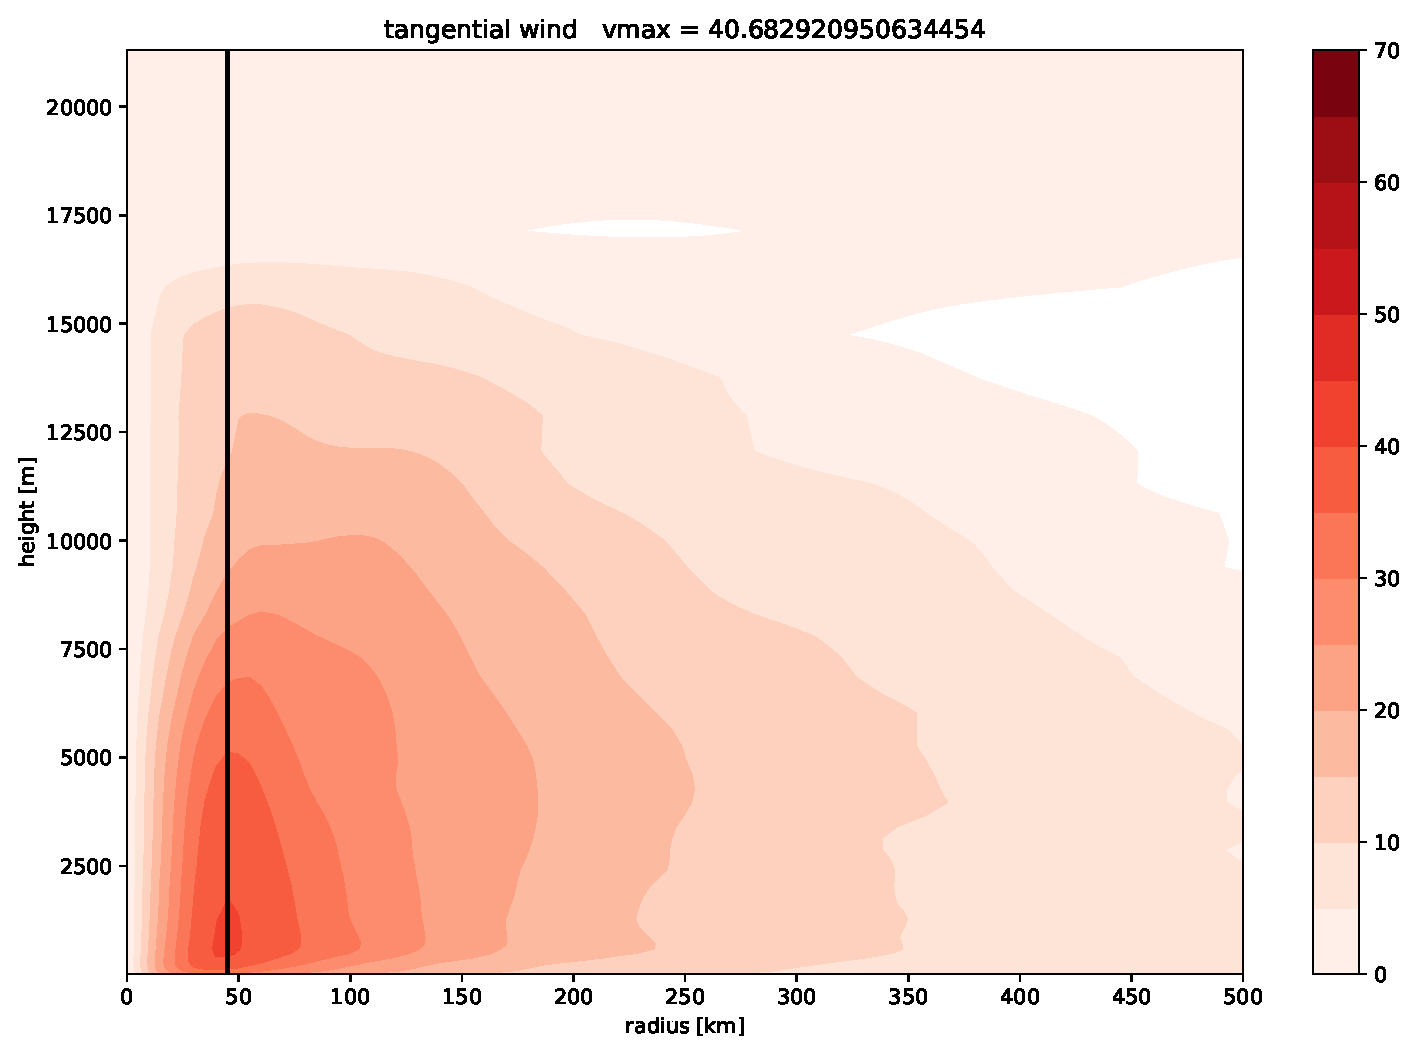
\includegraphics[width=0.75\linewidth]{img/tight09279566tanwind20130706T120000Z.eps}
\end{subfigure}
\begin{subfigure}{.5\linewidth}
    \centering
    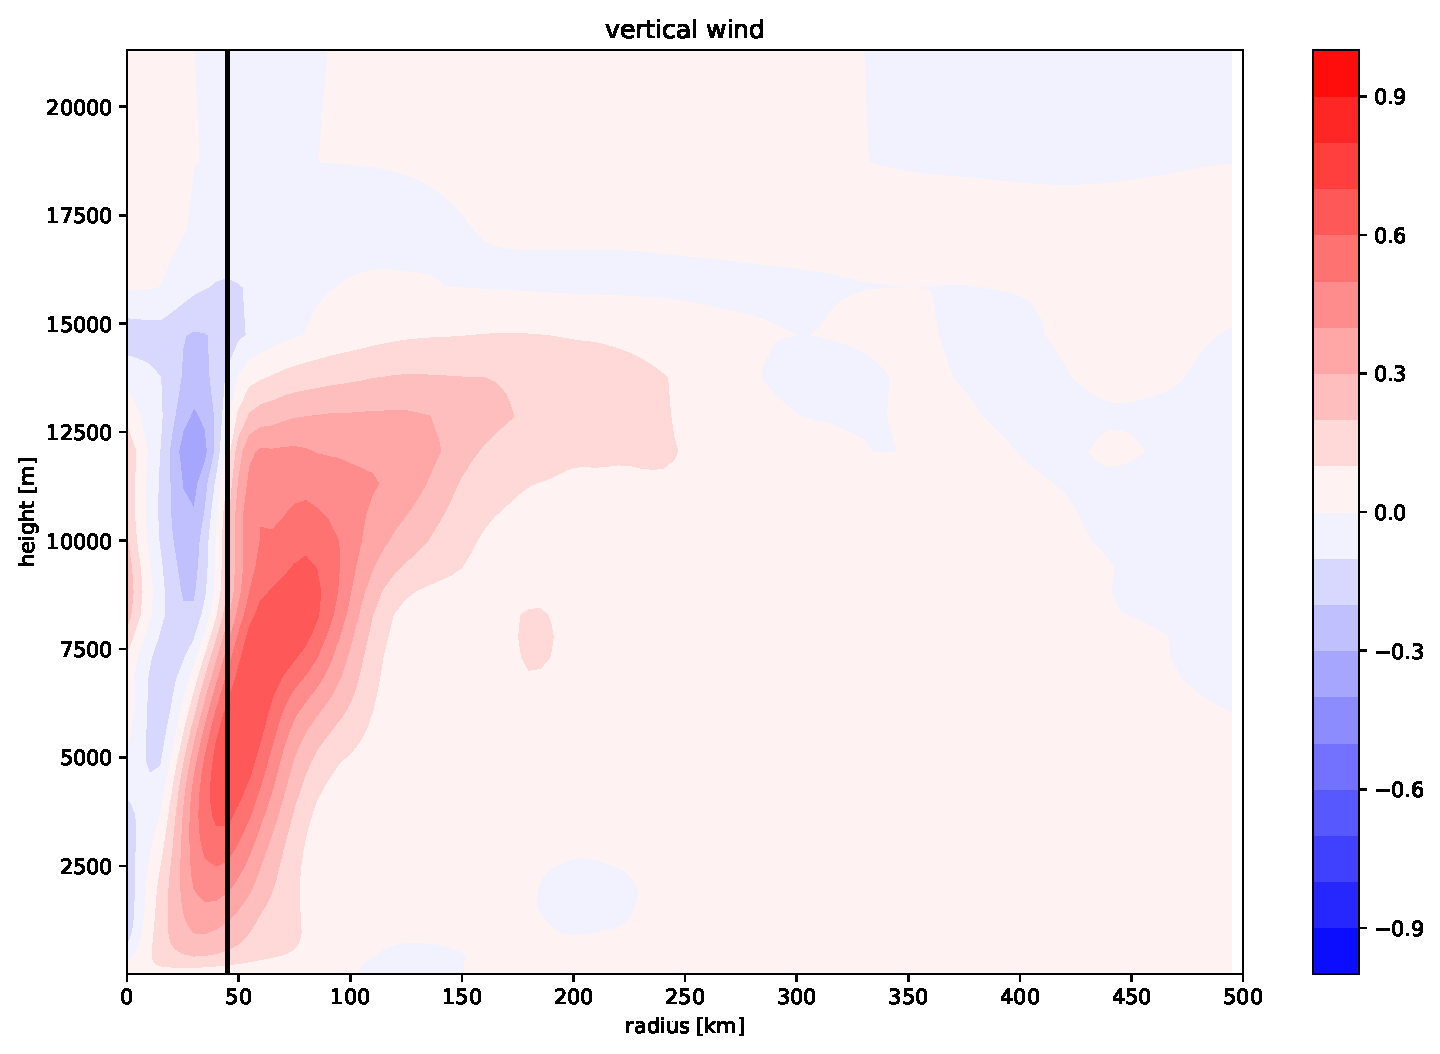
\includegraphics[width=0.75\linewidth]{img/tight09279566verwind20130706T120000Z.eps}
\end{subfigure}%
\begin{subfigure}{.5\linewidth}
    \centering
    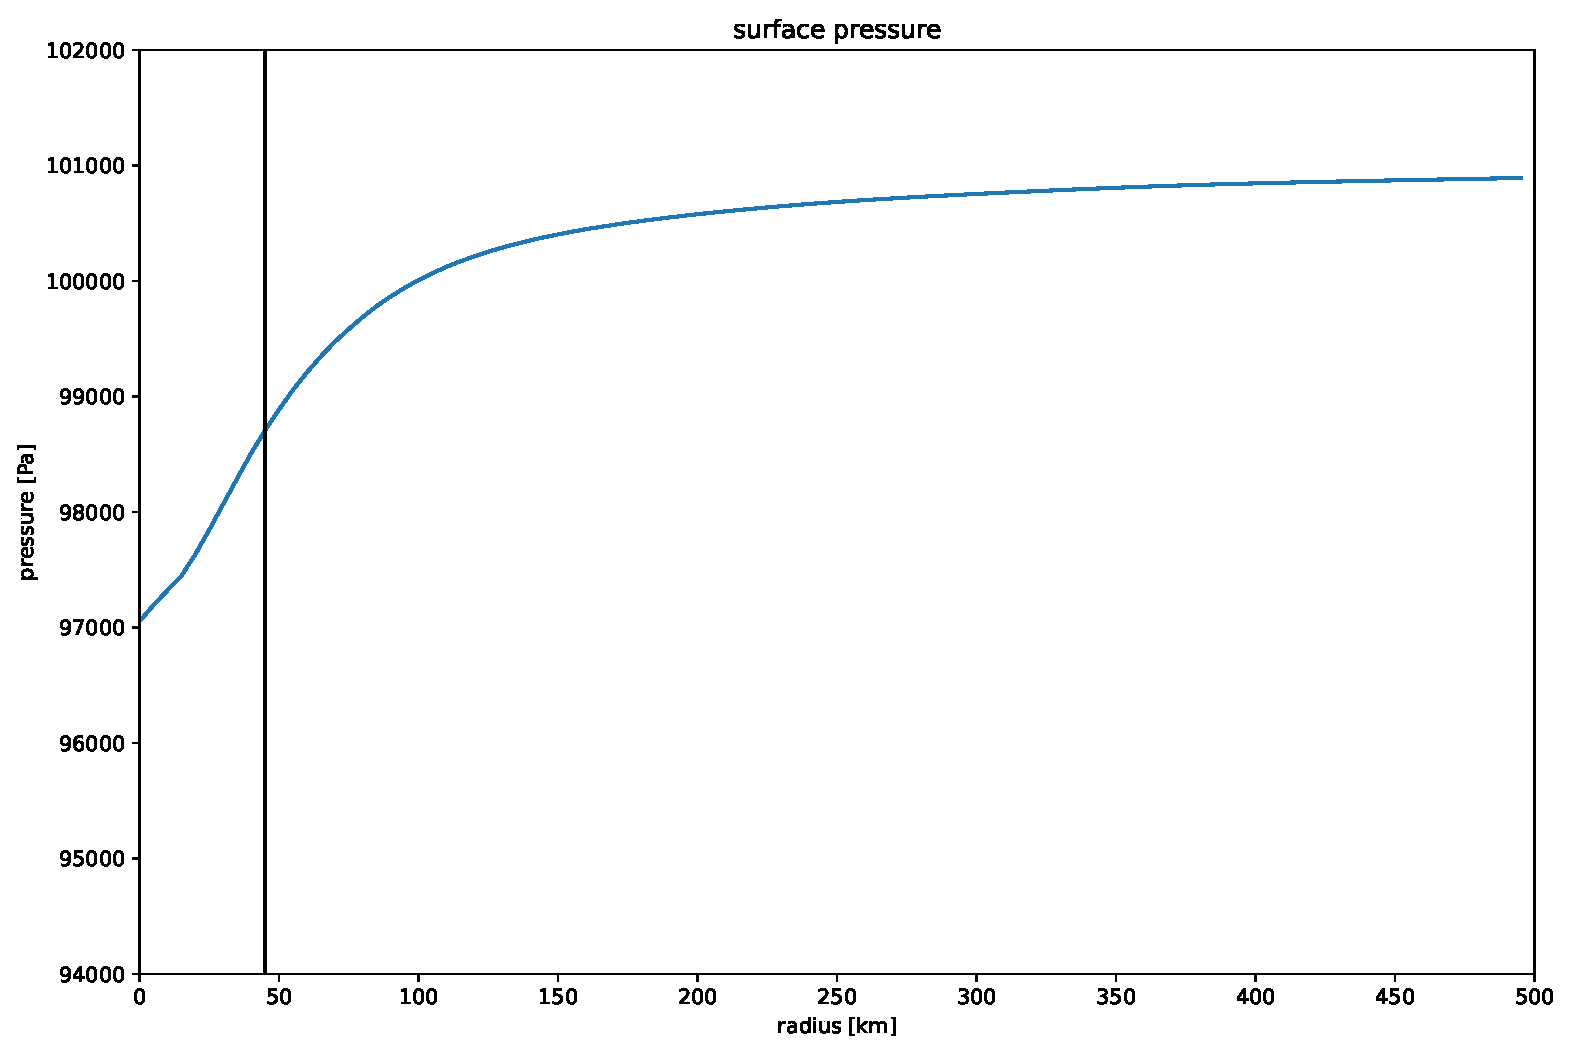
\includegraphics[width=0.75\linewidth]{img/tight09279566pres_msl20130706T120000Z.eps}
\end{subfigure}
\caption[short]{Azimuthal mean plots. From left to right and top to bottom: radial wind, tangential wind, vertical wind and sea level pressure.}
\end{figure}



\section{Variation of the Warm Core Criterion strength}
With the aim of understanding the impact of different warm core criteria strengths, the resulting cyclone distributions for a range of different \textbf{temdif}s were compared. As can be seen in Fig.~\ref{fig:temdif-analysis}, a weaker warm core criterion leads to a distribution with more lower intensity storms. When comparing with the absolute counts it can be seen that this is the result from weaker storms being tracked for lower \textbf{temdif}s. Logically for TCs of category 2 and upwards, no difference in the counts is observed. Furthermore for \textbf{temdif}s larger than \unit[1]{K}, no tropical depressions which correspond to category -1 are tracked. It can therefore be concluded that the warm core criterion can be used very efficiently to filter out noise if only strong TCs are of interest.
% TODO create plot that analyses category snapshots for tcs with max cat=2 and above
\begin{figure}[ht]
	\begin{minipage}[t]{0.48\textwidth}
		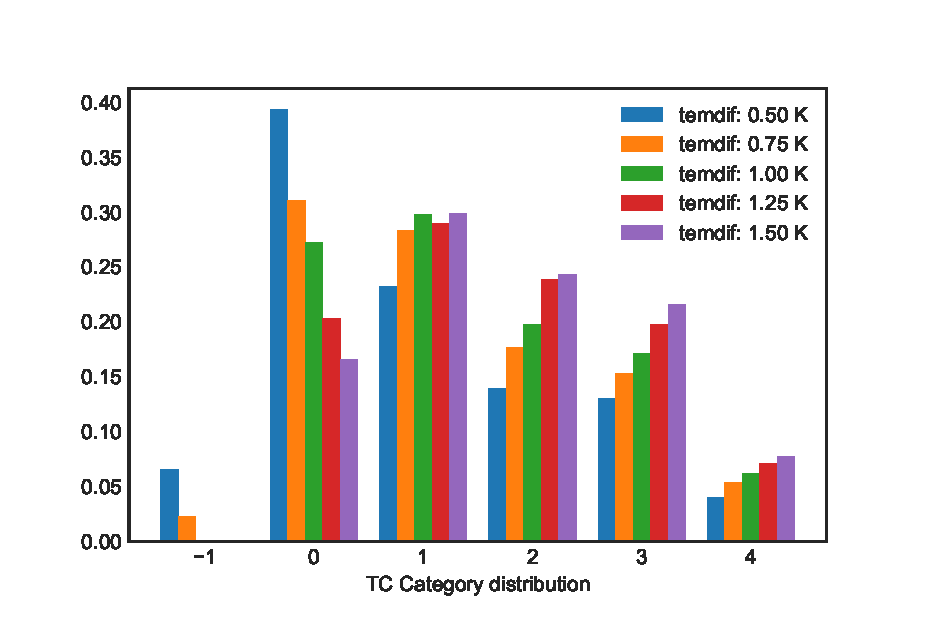
\includegraphics[width = \textwidth]{img/max_cat_distr_temdifs.eps}
	\end{minipage}
	\hfill
	\begin{minipage}[t]{0.48\textwidth}
		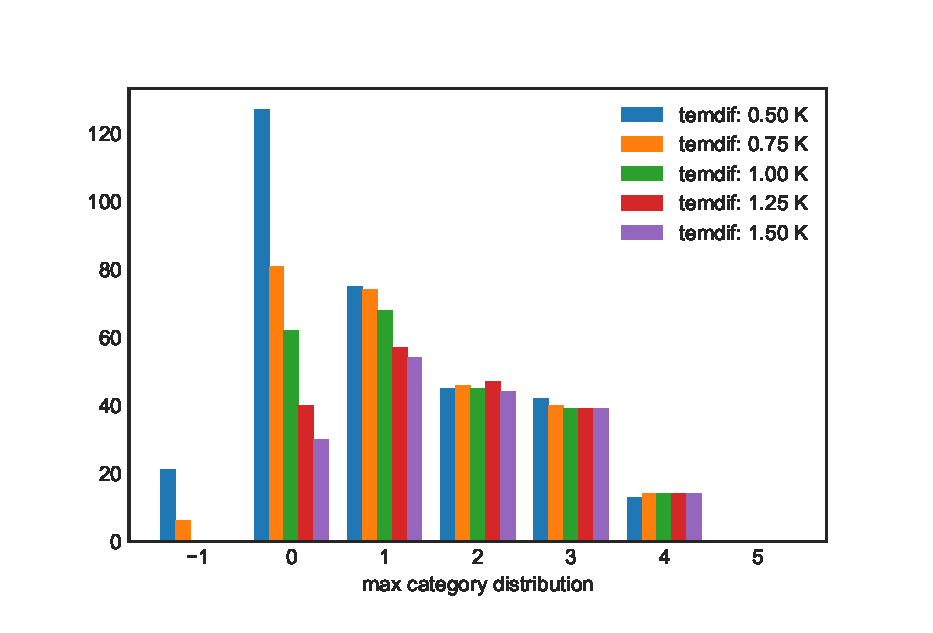
\includegraphics[width = \textwidth]{img/max_cat_counts_temdifs.eps}
	\end{minipage}
	\caption{Maximum TC category histograms for different \textbf{temdif} parameters. Each histogram on the left has unit norm. The right plot shows the absolute counts of TCs. The X-axis describes the TC categories as defined in Tab~\ref{tab:simpson-scale}.}
	\label{fig:temdif-analysis}
\end{figure}


\section{Comparison of the Warm Core Criterion and the Vorticity Threshold}\label{sec:warmcore-var}
In order to compare the importance of the warm core criterion with the vorticity threshold, TCs were tracked with parameter combinations of varying relative strength of the two criteria. To be concrete, all nine combinations of the parameters in Tab.~\ref{tab:vor-tem-comparison} were used.

\begin{table}[ht]
	\centering
	\begin{tabular}{|l|l|l|}
		\hline
		\textbf{parameter} & \textbf{unit} & \textbf{values}  \\ \hline
		slpdis             & m             & 100000           \\
		vormin             & 1/s           & 1e-6, 1e-5, 1e-4 \\
		temdif             & K             & 0.5, 1 ,1.5      \\
		temdis             & m             & 200000           \\ \hline
	\end{tabular}
	\caption{Parameter combinations used for the comparison}
	\label{tab:vor-tem-comparison}
\end{table}
% TODO really think about this and the max category influence of vorticity ask Bernhard
It was expected that the vorticity threshold should influence the distribution of tracked TCs only if a weak warm core criterion is applied. However, as can be seen in Fig.~\ref{fig:temdif-vormin-comp}, even with a very weak warm core criterion does the vorticity threshold not influence the storm intensity distributions. A comparison for different values of \textbf{temdif} and an analysis of the impact of the vorticity criterion on the storm lifetime, can be found in the Appendix.

\begin{figure}[ht]
	\centering
	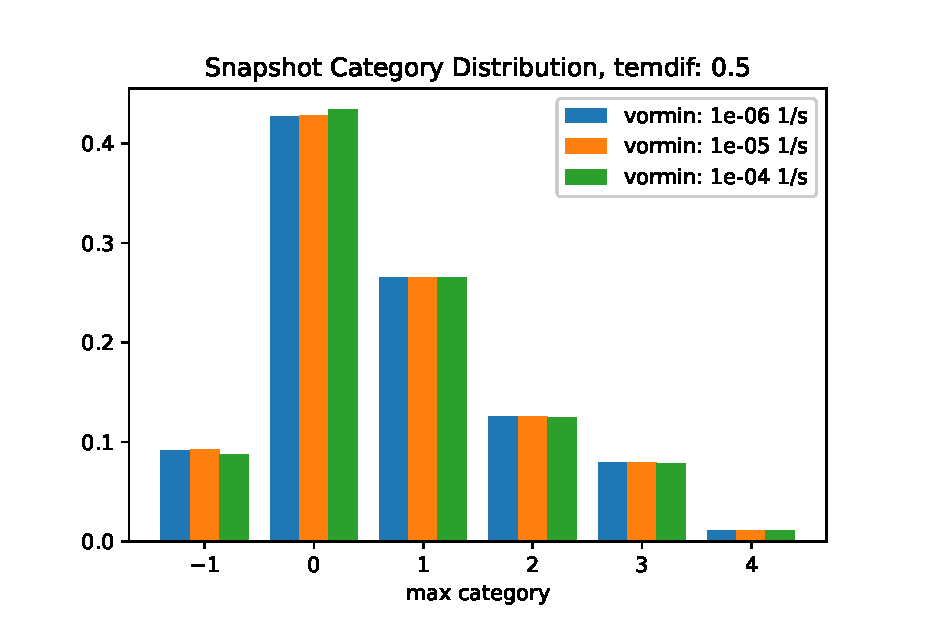
\includegraphics[width=0.7\textwidth]{img/curr_category_vortem05.eps}
	\caption{Snapshot category distribution for a weak warm core criterion and several vorticity thresholds}
	\label{fig:temdif-vormin-comp}
\end{figure}

\section{TC Genesis regions}
A direct consequence of the observations from Sec.~\ref{sec:warmcore-var} is that with a weaker warm core criterion the TCs can be found already when they have not had much time to intensify. This is relevant since from best track data it is expected that most TCs form in the main development region (MDR) which lies roughly between 10 -- 20 degree North and 20 -- 80 degree West. However, when checking the genesis spots and density in Fig.~\ref{fig:genesis-temdif1}, it can be seen that the MDR is not quite satisfied. When using a weaker warm core criterion 
\begin{figure}[ht]
	\centering
	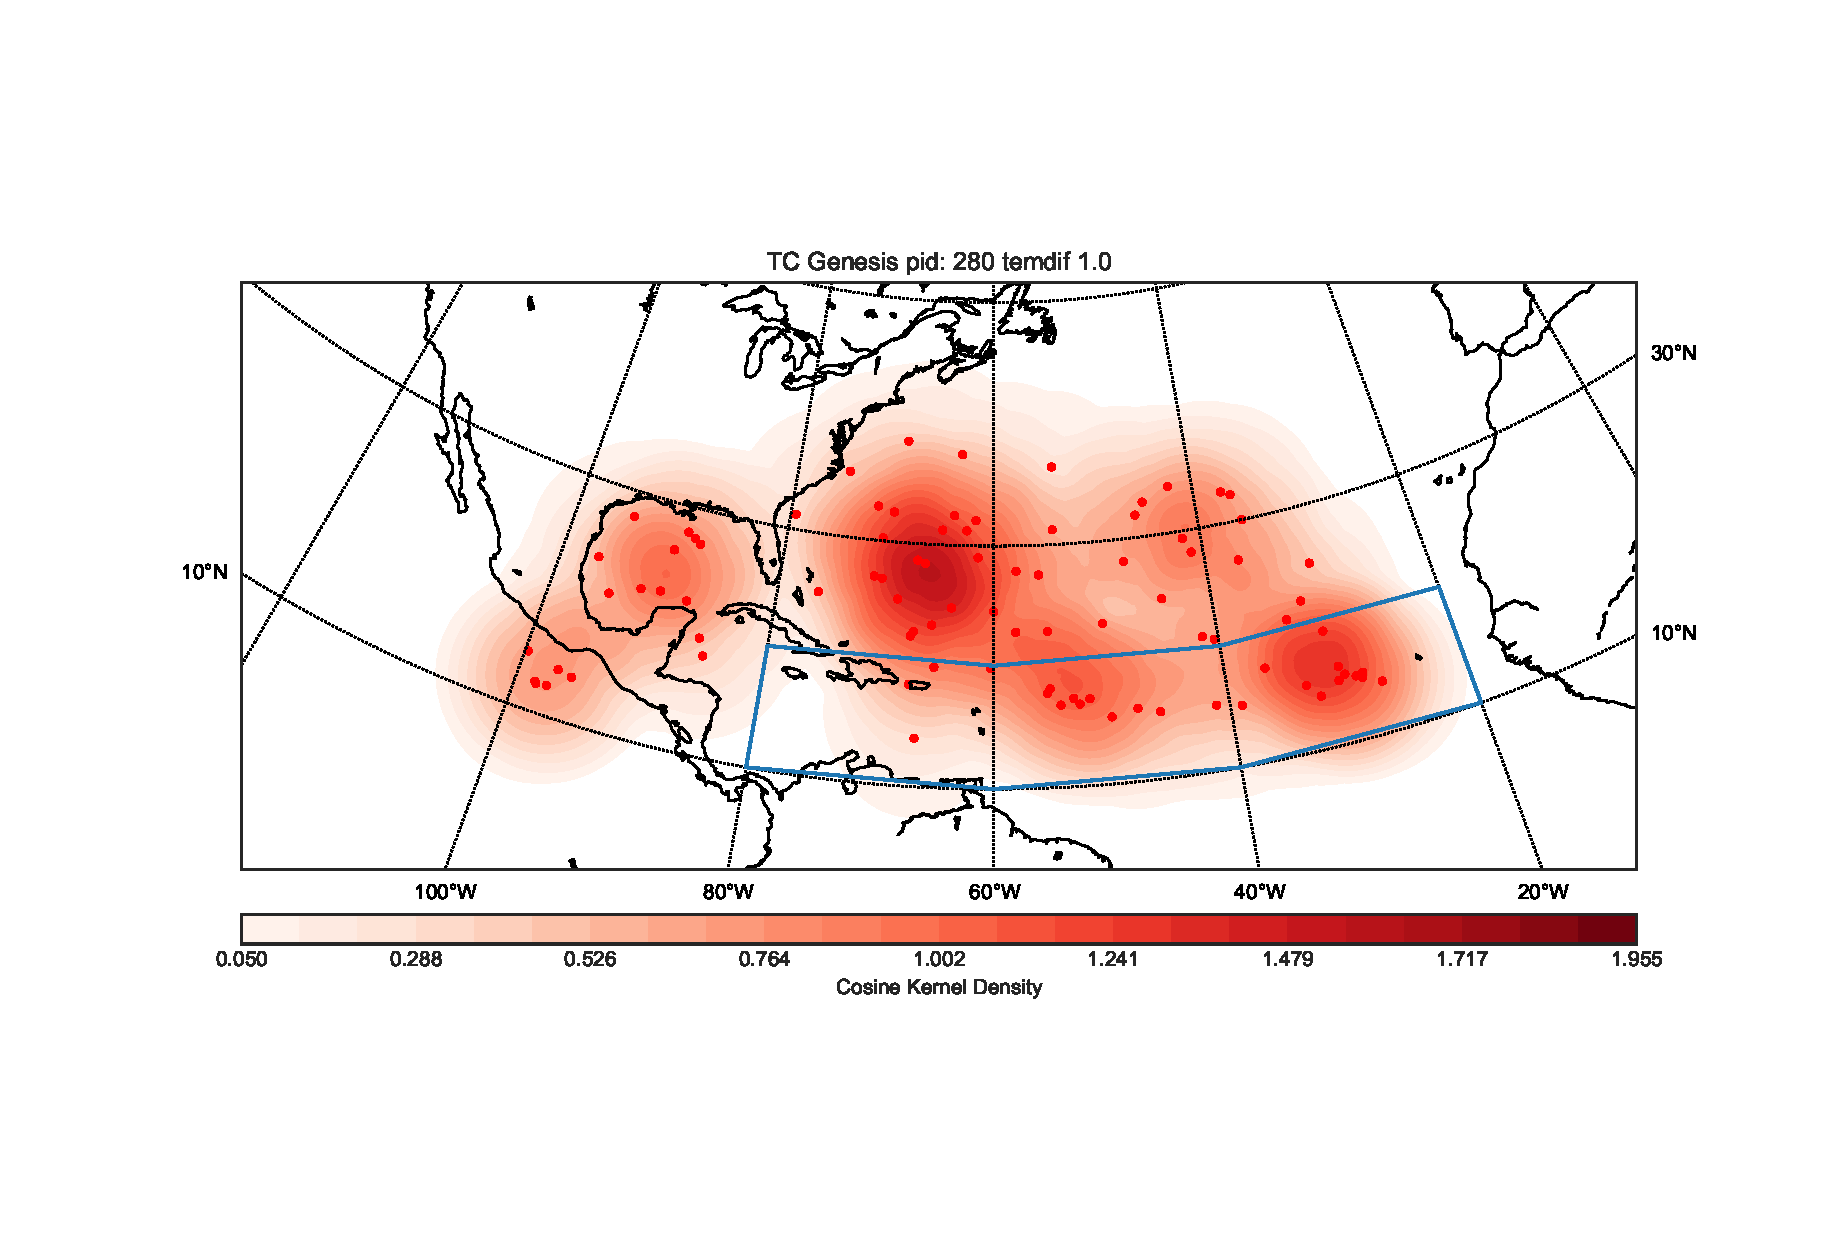
\includegraphics[width=0.7\textwidth]{img/genesis_plot_temdif1.eps}
	\caption{Genesis spots and density for a specific parameter combination.}
	\label{fig:genesis-temdif1}
\end{figure}
%TODO check counts instead of density
%\section{Importance of different criteria}

%\begin{enumerate}
%    \item which criteria have a large impact on the found tcs
%    \item what are interesting thresholds
%    \item Include fascinating plots
%\end{enumerate}


%\section{Recommended parameter combination}
%\begin{enumerate}
%    \item propose combination of parameters for robust search
%\end{enumerate}
